% Apresentação da Tese - Efeitos do Lobby no PE
% Beamer, pt-BR, ~15 min
% Compilar de Tese/tese_apresentacao/: pdflatex apresentacao.tex
% Figuras: ../imgs/ e ../figures/ (relativos a tese_apresentacao)

\documentclass[11pt,aspectratio=169]{beamer}
\usepackage[utf8]{inputenc}
\usepackage[T1]{fontenc}
\usepackage[brazilian,provide=*]{babel}
\usepackage{amsmath,amssymb}
\usepackage{graphicx}
\usepackage{url}
\usepackage{natbib}
\setcitestyle{authoryear,round,citesep={;}}

\usetheme{Madrid}
\usecolortheme{default}
\setbeamertemplate{navigation symbols}{}

\title{Mensurando os Efeitos do Lobby no Comportamento Parlamentar}
\subtitle{Painel com efeitos fixos no Parlamento Europeu}
\author{Acácio Vasconcelos Telechi}
\institute{Orientador: Prof.\ Dr.\ Alexsandro Eugênio Pereira \\[0.5em]
  UFPR -- Departamento de Ciência Política \\ PPG em Ciência Política}
\date{2025}

\begin{document}

% ---------------------------------------------------------------------------
\frame{\titlepage}

% ---------------------------------------------------------------------------
\begin{frame}{Objetivo e hipóteses}
  \textbf{Objetivo:} medir o efeito do lobby sobre o \textbf{comportamento parlamentar} no PE, operacionalizado como \textbf{Atividade Legislativa (AL)} = número de perguntas parlamentares 

  \vspace{0.8em}
  \textbf{Hipóteses:}
  \begin{itemize}
    \item \textbf{H1:} Maior pressão de lobby $\Rightarrow$ maior AL no domínio.
    \item \textbf{H2:} Lobby de organizações empresariais tende a aumentar mais a AL (em comparação com outros atores).
    \item \textbf{H3:} Em temas mais salientes, lobby não empresarial tende a aumentar mais a AL (em comparação com lobby empresarial).
  \end{itemize}
\end{frame}

% ---------------------------------------------------------------------------
\begin{frame}{Definições}
  \textbf{Lobby:}\\[0.3em]
  \textit{O exercício de influência sobre a atividade legislativa realizado por atores interessados em um ambiente marcado por diferenças de recursos.}

  \vspace{0.8em}
  \textbf{Comportamento parlamentar / Atividade Legislativa (AL):}\\[0.3em]
  \textit{O nível de envolvimento exibido por um parlamentar em um domínio político específico.}
  \vspace{0.5em}
\end{frame}

% ---------------------------------------------------------------------------
\begin{frame}{Revisão da literatura (brevíssima)}
  \begin{itemize}
    \item Literatura sobre \textbf{efeitos do lobby}: fragmentada, resultados mistos \citep{de_figueiredo_advancing_2014, baumgartner2009lobbying, mahoney_lobbying_2007}.
    \item \textbf{Desafios de identificação:} viés de seleção, variáveis omitidas, múltiplos canais, persistência temporal.
  \end{itemize}
  \vspace{0.6em}
  \textbf{Contribuição desta tese:}
  \begin{itemize}
    \item Cadeia causal \textbf{curta}: lobby $\to$ comportamento parlamentar (não resultado de política).
    \item Dados \textbf{públicos}: reuniões registradas (Registo de Transparência do PE).
    \item Modelo com \textbf{efeitos fixos de alta dimensão} para identificação causal.
  \end{itemize}
\end{frame}

% ---------------------------------------------------------------------------
\begin{frame}{DAG: comportamento parlamentar e efeitos do lobby}
  \begin{center}
    \IfFileExists{../imgs/DAG_v2.png}{%
      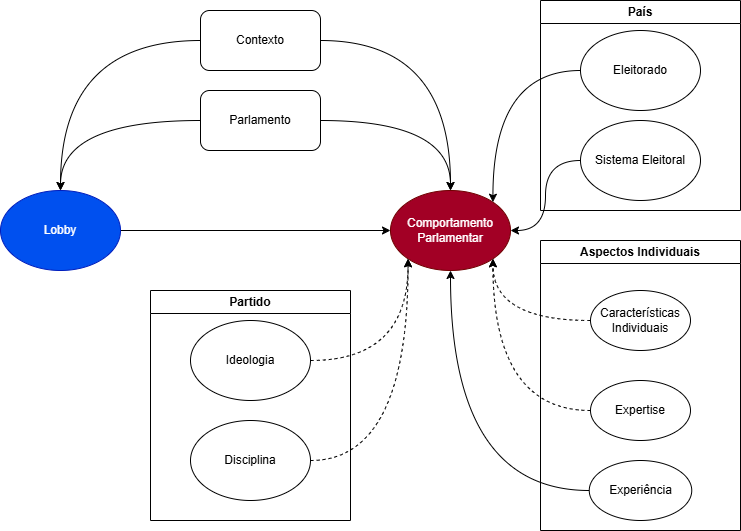
\includegraphics[width=0.6\textwidth]{../imgs/DAG_v2.png}%
    }{%
      \fbox{\parbox{0.7\textwidth}{\centering\vspace{2cm}Inserir figura \texttt{imgs/DAG\_v2.png}\\[0.5em](DAG: Lobby $\to$ Comportamento parlamentar; confundidores: Contexto, Parlamento, País, Partido, Aspectos individuais)\vspace{2cm}}}
    }
  \end{center}
  \vspace{0.3em}
  \small Fonte: autor (2025). Relações causais entre lobby, comportamento parlamentar e confundidores.
\end{frame}

% ---------------------------------------------------------------------------
\begin{frame}{Fundamentação teórica do DAG -- três dimensões do comportamento}
  \scriptsize
  \begin{tabular}{p{0.11\textwidth}p{0.45\textwidth}p{0.38\textwidth}}
    \hline
    \textbf{Dimensão} & \textbf{Fundamentação teórica} & \textbf{Referências} \\
    \hline
    \textbf{Contexto} & Ambiente político, econômico e social: crises, opinião pública, eventos midiáticos e ciclos eleitorais intensificam mobilização de interesses e alteram a agenda legislativa, gerando correlação espúria entre lobby e comportamento. & \citep{mahoney_lobbying_2007, mahoney2008brussels, baumgartner2010agendas, jones2005politics} \\
    \hline
    \textbf{Parlamento} & Regras, agenda da liderança, prazos de tramitação e estrutura das comissões afetam quem é alvo de lobby e o comportamento (ex.: relatório em tramitação atrai lobistas ao relator e aumenta sua atividade). & \citep{marshall2010lobby, kluver2015legislative, coen2019legislative} \\
    \hline
    \textbf{País} & Sistema eleitoral e eleitorado criam incentivos (voto pessoal $\to$ visibilidade; lista fechada $\to$ disciplina). Tamanho e diversidade do eleitorado moldam \textit{vote-seeking}. & \citep{mayhew2004congress, samuels1997determinantes, carey2007competing, willumsen_electoral_2019} \\
    \hline
    \textbf{Partido} & Ideologia como regras informais; disciplina via sanções e recompensas (seleção, cargos, recursos). Variáveis latentes. & \citep{hix2004electoral, helmke2012informal, carey2007competing, bressanelli2016impact} \\
    \hline
    \textbf{Aspectos individuais} & Expertise (ocupação prévia) e experiência (mandato, cargos) influenciam atuação e \textit{career-seeking}; comitês e trajetória partidária. & \citep{burden2015personal, damgaard1980dilemma, daniel2015career, chiru2020loyal} \\
    \hline
  \end{tabular}
  \vspace{0.3em}
  \scriptsize Mecanismo causal subjacente: troca \citep{de_figueiredo_advancing_2014}
\end{frame}

% % ---------------------------------------------------------------------------
% \begin{frame}{Leitura do DAG e estratégia de identificação}
%   \textbf{Relação de interesse:} seta \textbf{Lobby $\to$ Comportamento parlamentar} (efeito causal $\beta$).

%   \vspace{0.5em}
%   \textbf{Confundidores (backdoor paths):}
%   \begin{itemize}
%     \item \textbf{Contexto:} crises, opinião pública, ciclos eleitorais.
%     \item \textbf{Parlamento:} agenda, comissões, relatórios.
%     \item \textbf{Três dimensões do comportamento:} País (sistema eleitoral, eleitorado), Partido (ideologia, disciplina), Aspectos individuais (expertise, cargos).
%   \end{itemize}
%   \vspace{0.5em}
%   \textbf{Estratégia:} bloquear esses caminhos com \textbf{efeitos fixos} país$\times$tempo, partido$\times$tempo, domínio$\times$tempo e efeito fixo de membro; identificação por variação \textit{within} MEP ao longo do tempo.
% \end{frame}

% ---------------------------------------------------------------------------
\begin{frame}{Metodologia -- modelo}
  \textbf{Variáveis:}
  \begin{itemize}
    \item VD: $AL_{idt}$ = contagem de perguntas (MEP $i$, domínio $d$, mês $t$).
    \item Tratamento: $L_{idt}$ = contagem de reuniões de lobby.
  \end{itemize}
  \vspace{0.5em}
  \textbf{Modelo PPML (equação principal):}
  \begin{equation*}
    AL_{idt} = \beta L_{idt} + \gamma_{ct} + \lambda_{pt} + \theta_{dt} + X'_{it}\delta + \epsilon_{idt}
  \end{equation*}
  \small
  \begin{itemize}
    \item $\gamma_{ct}$: efeito fixo país$\times$tempo \quad $\lambda_{pt}$: efeito fixo partido$\times$tempo \quad $\theta_{dt}$: efeito fixo domínio$\times$tempo
    \item $X'_{it}$: controles (ex.: cargos de liderança)
  \end{itemize}
  \normalsize
  Inferência: erros clusterizados em domínio$\times$tempo e membro.
\end{frame}

% ---------------------------------------------------------------------------
\begin{frame}{Resultados -- Hipótese 1}
  \textbf{Maior lobby $\Rightarrow$ maior atividade parlamentar.}
  \begin{itemize}
    \item Coeficiente de reuniões \textbf{positivo} e significativo: $\approx$ 2,5\% de aumento nas perguntas por reunião adicional (especificação linear).
    \item \textbf{Retornos marginais decrescentes} (termo quadrático negativo); ponto de inflexão em $\approx$ 12 reuniões.
    \item Efeito positivo em (quase) todos os domínios temáticos.
  \end{itemize}
  \vspace{0.5em}
  Conclusão: H1 corroborada; robustez em especificações alternativas.
\end{frame}

% ---------------------------------------------------------------------------
\begin{frame}{Resultados -- Hipótese 2}
  \textbf{Persuasão por reunião:} ONGs $>$ empresas (uma reunião de ONG gera mais perguntas, em média).
  \vspace{0.4em}
  \textbf{Efeito total = Acesso $\times$ Persuasão} (modelo em duas etapas: Binomial Negativa + PPML):
  \begin{itemize}
    \item Abaixo de $\approx$ \$8,8 milhões de orçamento: efeito total das ONGs maior.
    \item Acima de $\approx$ \$40 milhões: efeito agregado das empresas substancialmente maior.
  \end{itemize}
  \vspace{0.4em}
  Recursos financeiros convertem-se em \textbf{acesso}; ONGs têm maior \textbf{eficiência por reunião}. H2 corroborada com nuance: vantagem empresarial depende de recursos.
\end{frame}

% ---------------------------------------------------------------------------
\begin{frame}{Resultados -- Hipótese 3}
  \textbf{Saliência temática:} em temas mais salientes, o efeito do lobby \textbf{diminui para todos} os atores.
  \vspace{0.4em}
  \textbf{Heterogeneidade:} efeito das ONGs \textbf{mais resiliente}; em alta saliência, efeito de empresas e outros $\approx 0$, ONGs ainda positivas e significativas.
  \vspace{0.4em}
  Em temas mais salientes, lobby não empresarial é \textbf{relativamente} mais eficaz (resiliência ao escrutínio público). H3 corroborada.
\end{frame}

% ---------------------------------------------------------------------------
\begin{frame}{Conclusão}
  \textbf{Síntese:}
  \begin{itemize}
    \item H1: Lobby aumenta a atenção legislativa (com retornos marginais decrescentes).
    \item H2: Influência agregada das empresas superior quando há muitos recursos; ONGs com maior persuasão por reunião.
    \item H3: Saliência reduz influência de todos; ONGs relativamente mais eficazes sob escrutínio.
  \end{itemize}
  \vspace{0.4em}
  \textbf{Implicações:} influência no PE = ecossistema (recursos, tipo de ator, saliência); informação credível como moeda; escrutínio público como contrapeso.
  \vspace{0.4em}
  \small Limitações: AL não esgota o comportamento parlamentar; dados do Registo de Transparência.
\end{frame}

% ---------------------------------------------------------------------------
\begin{frame}[allowframebreaks]{Referências}
  \bibliographystyle{apalike}
  \bibliography{../refs}
\end{frame}

% ---------------------------------------------------------------------------
\begin{frame}{}
  \begin{center}
    \Large Obrigado!
    \vspace{1em}
    \normalsize
    \textbf{Mensurando os Efeitos do Lobby no Comportamento Parlamentar} \\[0.3em]
    Acácio Vasconcelos Telechi \\[0.3em]
    \url{https://github.com/AcacioTelechi/thesis-lobbying-effects}
  \end{center}
\end{frame}

\end{document}
